\documentclass{article}
\usepackage{graphicx}
\usepackage{hyperref}
\begin{document}
\title{Lösung: Logische Uhren und happens-before}
\maketitle

\section{Einführung}
In diesem Dokument beschäftigen wir uns mit einer Sequenz von Nachrichten, die zwischen vier Knoten in einem Netzwerk ausgetauscht werden. Die Sequenz ist im folgenden Diagramm dargestellt:

\begin{figure}[h]
\centering
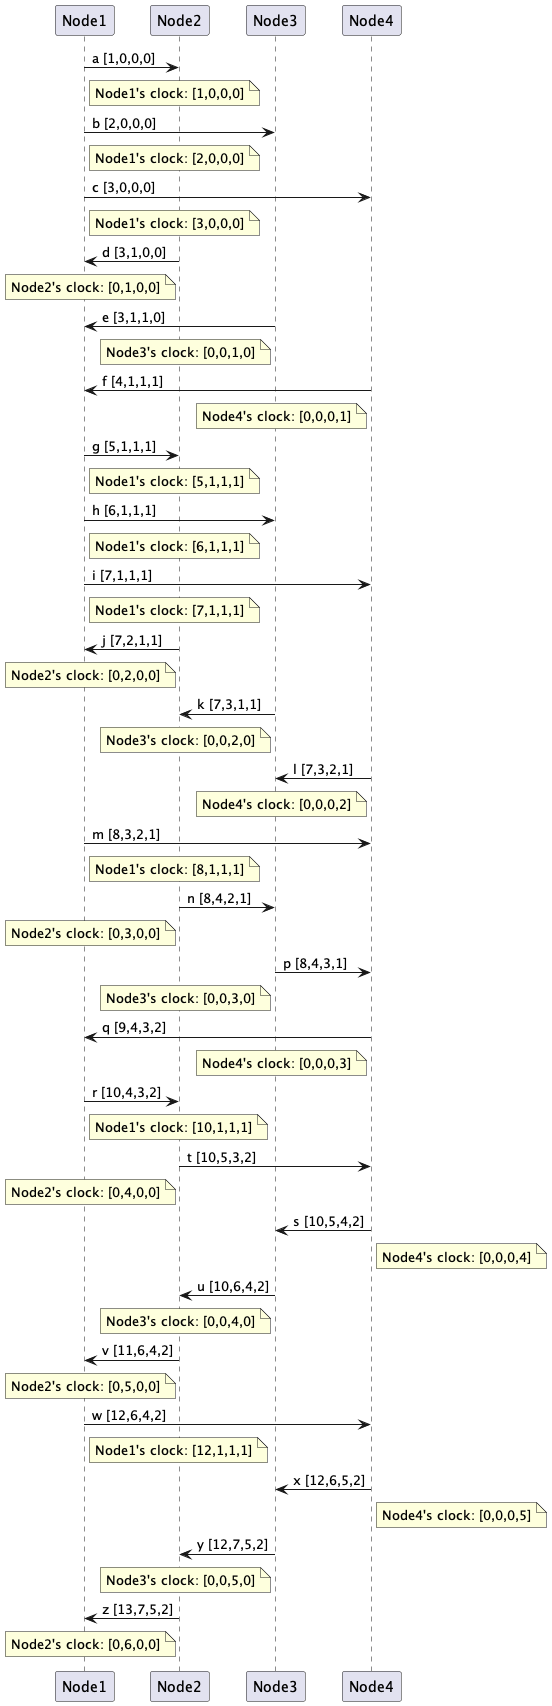
\includegraphics[width=0.65\textwidth]{../../fig/uml/clock_exam_concurrent.png}
\caption{Sequenzdiagramm der Nachrichten}
\label{fig:sequenzdiagramm}
\end{figure}

\section{Aufgaben und Antworten}

\subsection{Aufgabe 1}
\textit{Beschreiben Sie die Nachrichtensequenz von Node1 zu den anderen Knoten. Geben Sie die Reihenfolge der Nachrichten an.}

Antwort: Node1 sendet zunächst die Nachrichten `a` an Node2, `b` an Node3 und `c` an Node4. Nachdem Node1 die Antworten `d` von Node2, `e` von Node3 und `f` von Node4 erhält, sendet Node1 weitere Nachrichten `g` an Node2, `h` an Node3 und `i` an Node4. Während der konkurrierenden Phase sendet Node1 die Nachricht `m` an Node4 und später `r` an Node2. Schließlich sendet Node1 die Nachrichten `v`, `w` und `z` an Node4, Node2 und Node4 in dieser Reihenfolge.

\subsection{Aufgabe 2}
\textit{Welche Nachrichten sind konkurrierend? Was bedeutet das in diesem Kontext?}

Antwort: Die Nachrichten `j`, `k`, `l`, `m`, `n`, `p`, `q`, `r` und `t` sind konkurrierend. Das bedeutet, dass sie gleichzeitig und in keiner spezifischen Reihenfolge gesendet oder empfangen werden können. 

\subsection{Aufgabe 3}
\textit{Beschreiben Sie den Nachrichtenfluss, der mit der Nachricht `j` beginnt und mit der Nachricht `t` endet. Welche Knoten sind beteiligt?}

Antwort: Der Nachrichtenfluss beginnt mit Node2, der die Nachricht `j` an Node1 sendet. Dann sendet Node3 die Nachricht `k` an Node2 und Node4 sendet die Nachricht `l` an Node3. Node1 sendet die Nachricht `m` an Node4 und Node2 sendet die Nachricht `n` an Node3. Dann sendet Node3 die Nachricht `p` an Node4 und Node4 sendet die Nachricht `q` an Node1. Schließlich sendet Node1 die Nachricht `r` an Node2 und Node2 sendet die Nachricht `t` an Node4. 

\subsection{Aufgabe 4}
\textit{Erweitern Sie das Sequenzdiagramm um zwei weitere Knoten, die Nachrichten mit den Knoten 1 bis 4 austauschen. Was ändert sich in Bezug auf die Komplexität des Netzwerks?}

Antwort: Durch das Hinzufügen von zwei weiteren Knoten erhöht sich die Komplexität des Netzwerks signifikant. Jeder neue Knoten kann potenziell mit jedem vorhandenen Knoten kommunizieren, was die Anzahl der möglichen Nachrichtenpfade erhöht. Außerdem müssen wir die zusätzliche Konkurrenz zwischen Nachrichten, die von oder zu den neuen Knoten gesendet werden, berücksichtigen. Es kann auch mehr Synchronisation erforderlich sein, um sicherzustellen, dass die Nachrichten korrekt empfangen und verarbeitet werden.

\subsection{Aufgabe 5}
\textit{Schreiben Sie ein kurzes Programm in einer Programmiersprache Ihrer Wahl, das diesen Nachrichtenaustausch simuliert. Was sind die Herausforderungen bei der Simulation dieser Sequenz?}

Antwort: Eine mögliche Herausforderung bei der Simulation dieser Sequenz könnte die korrekte Modellierung der konkurrierenden Nachrichten sein. In einer realen Situation könnten diese Nachrichten zu beliebigen Zeiten und in beliebiger Reihenfolge eintreffen, was schwer vorherzusagen und zu kontrollieren sein kann. Darüber hinaus könnte die korrekte Behandlung und Synchronisation von eingehenden Nachrichten auf jedem Knoten eine Herausforderung sein, insbesondere in Situationen, in denen mehrere Nachrichten fast gleichzeitig eintreffen.

\end{document}
